\chapter{Images as Arrays}
\label{ch:lesson01}

A digital image is a 2D grid of numbers. This chapter builds a small image from scratch with NumPy, examines how grayscale and color images are represented, and displays them.

\section{A grayscale image is a 2D array}

Each entry is a pixel intensity. For an 8-bit image, pixel values range from 0 (black) to 255 (white), as in Figure~\ref{fig:l01-1}.

\begin{lstlisting}
im = np.zeros((100, 100), dtype=np.uint8)
im[20:80, 20:80] = 255   # a white square on a black background
\end{lstlisting}

\begin{figure}[h]
\centering
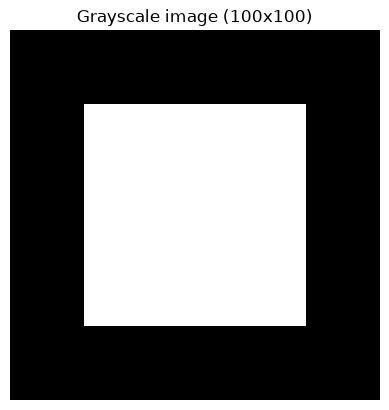
\includegraphics[width=0.35\textwidth]{figures/lesson01_fig01.png}
\caption{A $100\times100$ grayscale array with a white square.}
\label{fig:l01-1}
\end{figure}

\subsection*{Simple pixel-level operations}

Because an image is just an array of numbers, standard NumPy operations apply directly, e.g., inverting intensities with \code{im\_inv = 255 - im} (Figure~\ref{fig:l01-2}).

\begin{figure}[h]
\centering
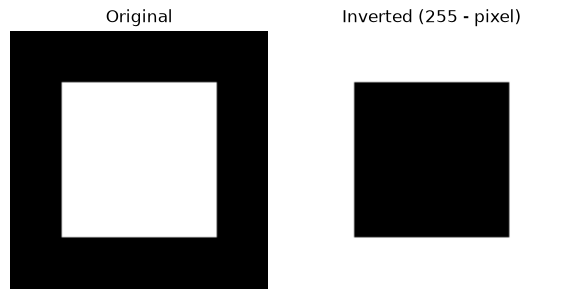
\includegraphics[width=0.6\textwidth]{figures/lesson01_fig02.png}
\caption{Inversion is a single elementwise array operation.}
\label{fig:l01-2}
\end{figure}

\section{A color image is a 3D array}

An image's dimensions are \code{(height, width, channels)} --- the output of \code{array.shape}. The \textbf{first} axis selects the row (moving down the image, i.e., $y$), the \textbf{second} axis selects the column (moving across, i.e., $x$); the \textbf{third} axis selects the color channel (red, green, or blue). By convention, the origin is the top-left corner.

\begin{warningbox}
Even though \code{array.shape} and NumPy indexing use \code{(row, column)} = \code{(y, x)} ordering, many OpenCV functions that take points or sizes --- \code{cv2.circle}, \code{cv2.rectangle}, \code{cv2.resize}, \code{cv2.warpAffine}'s \code{dsize}, etc. --- expect the \emph{opposite} order, \code{(x, y)} or \code{(width, height)}. This reversal is a common source of bugs; always check a function's argument order rather than assuming it matches array shape.
\end{warningbox}

\begin{lstlisting}
imc = np.zeros((50, 100, 3), dtype=np.uint8)
imc[:, :, 0] = 255          # red channel on for the whole image
imc[10:40, 20:80, 1] = 255  # add green in the middle -> looks yellow
\end{lstlisting}

The result is shown in Figure~\ref{fig:l01-3}.

\begin{figure}[h]
\centering
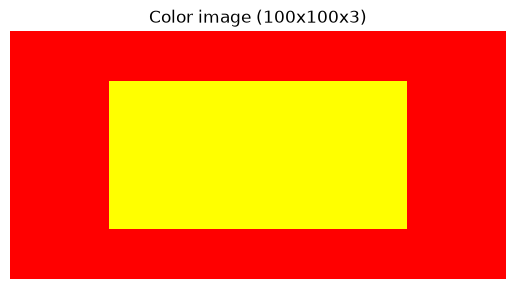
\includegraphics[width=0.55\textwidth]{figures/lesson01_fig03.png}
\caption{Red + green renders as yellow.}
\label{fig:l01-3}
\end{figure}

\subsection*{Colors are typically in RGB order}

To illustrate channel order, build a tiny image out of the six \emph{psychological primaries} --- the six hues (black, white, red, yellow, green, blue) the human visual system treats as elementary (Figure~\ref{fig:l01-4}).

\begin{figure}[h]
\centering
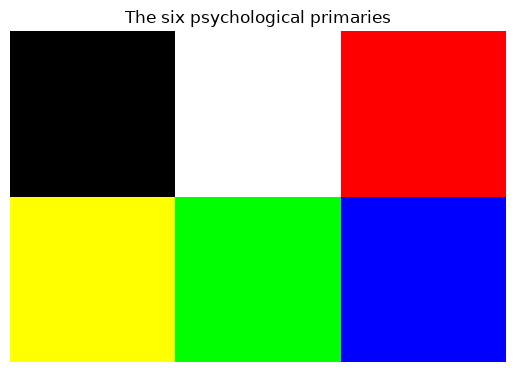
\includegraphics[width=0.5\textwidth]{figures/lesson01_fig04.png}
\caption{The six psychological primaries as a $2\times3$ RGB image.}
\label{fig:l01-4}
\end{figure}

Slicing the first axis selects whole rows (a horizontal band); slicing the second axis selects whole columns (a vertical band), as Figure~\ref{fig:l01-5} shows directly.

\begin{notebox}
A bare integer index (\code{im[0, :, :]}) \emph{drops} that axis entirely, turning shape \code{(1, 3, 3)} into \code{(3, 3)} --- \code{imshow} would then misread it as a $3\times3$ grayscale image rather than a 1-row RGB strip. Slicing with \code{0:1} keeps the axis alive as size 1.
\end{notebox}

\begin{figure}[h]
\centering
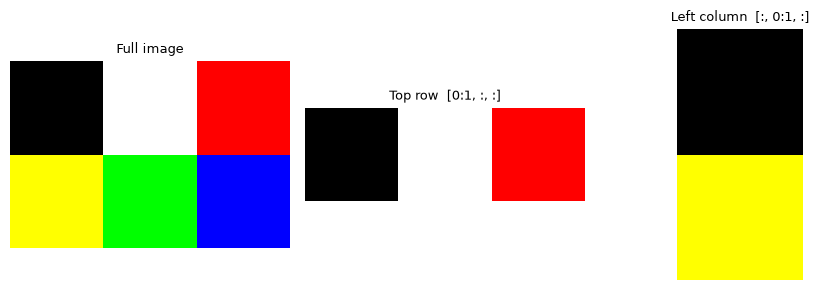
\includegraphics[width=0.75\textwidth]{figures/lesson01_fig05.png}
\caption{Slicing the first axis selects a row; the second axis, a column.}
\label{fig:l01-5}
\end{figure}

\section{Loading a real photo: BGR vs. RGB}

Every color image so far was constructed manually with channels in RGB order --- matching what Matplotlib's \code{plt.imshow} expects. Real photos, however, are loaded with OpenCV's \code{cv2.imread}, which reads (and writes) color images with channels in \textbf{BGR} order --- blue first, red last --- the opposite of the RGB order every other Python imaging library assumes. Handing a BGR array straight to \code{imshow} misinterprets the channels, producing a color-shifted image.

There are two equivalent ways to fix this:
\begin{enumerate}
  \item \textbf{Reverse the channel axis with NumPy indexing:} \code{img[:, :, ::-1]} turns \code{[B, G, R]} into \code{[R, G, B]} --- a plain array operation, no OpenCV function needed.
  \item \textbf{\code{cv2.cvtColor}:} OpenCV's general-purpose color-conversion function; \code{cv2.COLOR\_BGR2RGB} performs exactly the same channel swap, but is more explicit about \emph{why}, and is the idiomatic choice in OpenCV code (the same function also handles conversions that are not a simple reversal, e.g.\ to grayscale or HSV, in later lessons).
\end{enumerate}

\begin{lstlisting}
im_rgb1 = im_bgr[:, :, ::-1]
im_rgb2 = cv2.cvtColor(im_bgr, cv2.COLOR_BGR2RGB)
# np.array_equal(im_rgb1, im_rgb2) -> True: both fixes agree exactly
\end{lstlisting}

Figure~\ref{fig:l01-6} compares the raw BGR array against both fixes.

\begin{figure}[h]
\centering
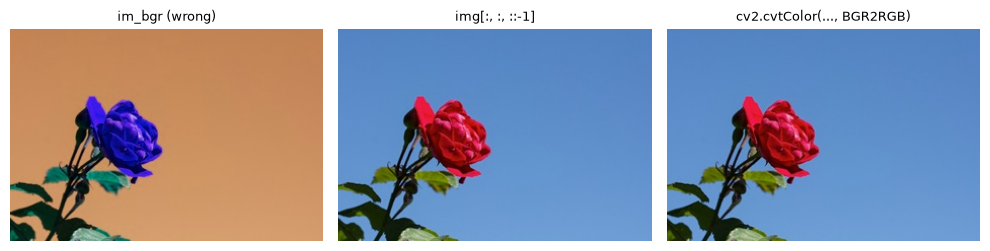
\includegraphics[width=0.85\textwidth]{figures/lesson01_fig07.png}
\caption{Left: BGR array shown directly (wrong colors). Center and right: the two equivalent fixes, in agreement. \attrib{Photo: \href{https://picryl.com}{Picryl}.}}
\label{fig:l01-6}
\end{figure}

\subsection*{Exercises}
\begin{enumerate}
  \item Modify the color image \code{imc} so the rectangle is cyan instead of yellow. Which channel(s) need to change?
  \item In the primaries image, slice out the \emph{bottom-right} block (blue) using row and column ranges, and confirm with \code{np.array\_equal} that it matches a fresh block filled with \code{(0, 0, 255)}.
  \item Load \code{rose.jpg} and print \code{im\_bgr[0, 0, :]} alongside \code{im\_rgb2[0, 0, :]}. Confirm by hand that the three numbers are the same three numbers, just reordered.
\end{enumerate}

\vfill
\fullcode{lesson01}{lesson01_images_as_arrays}
